\section{Diagram klas}

\subsection{Rysunek (diagram)}
\begin{figure}[!htb]
    \centering
    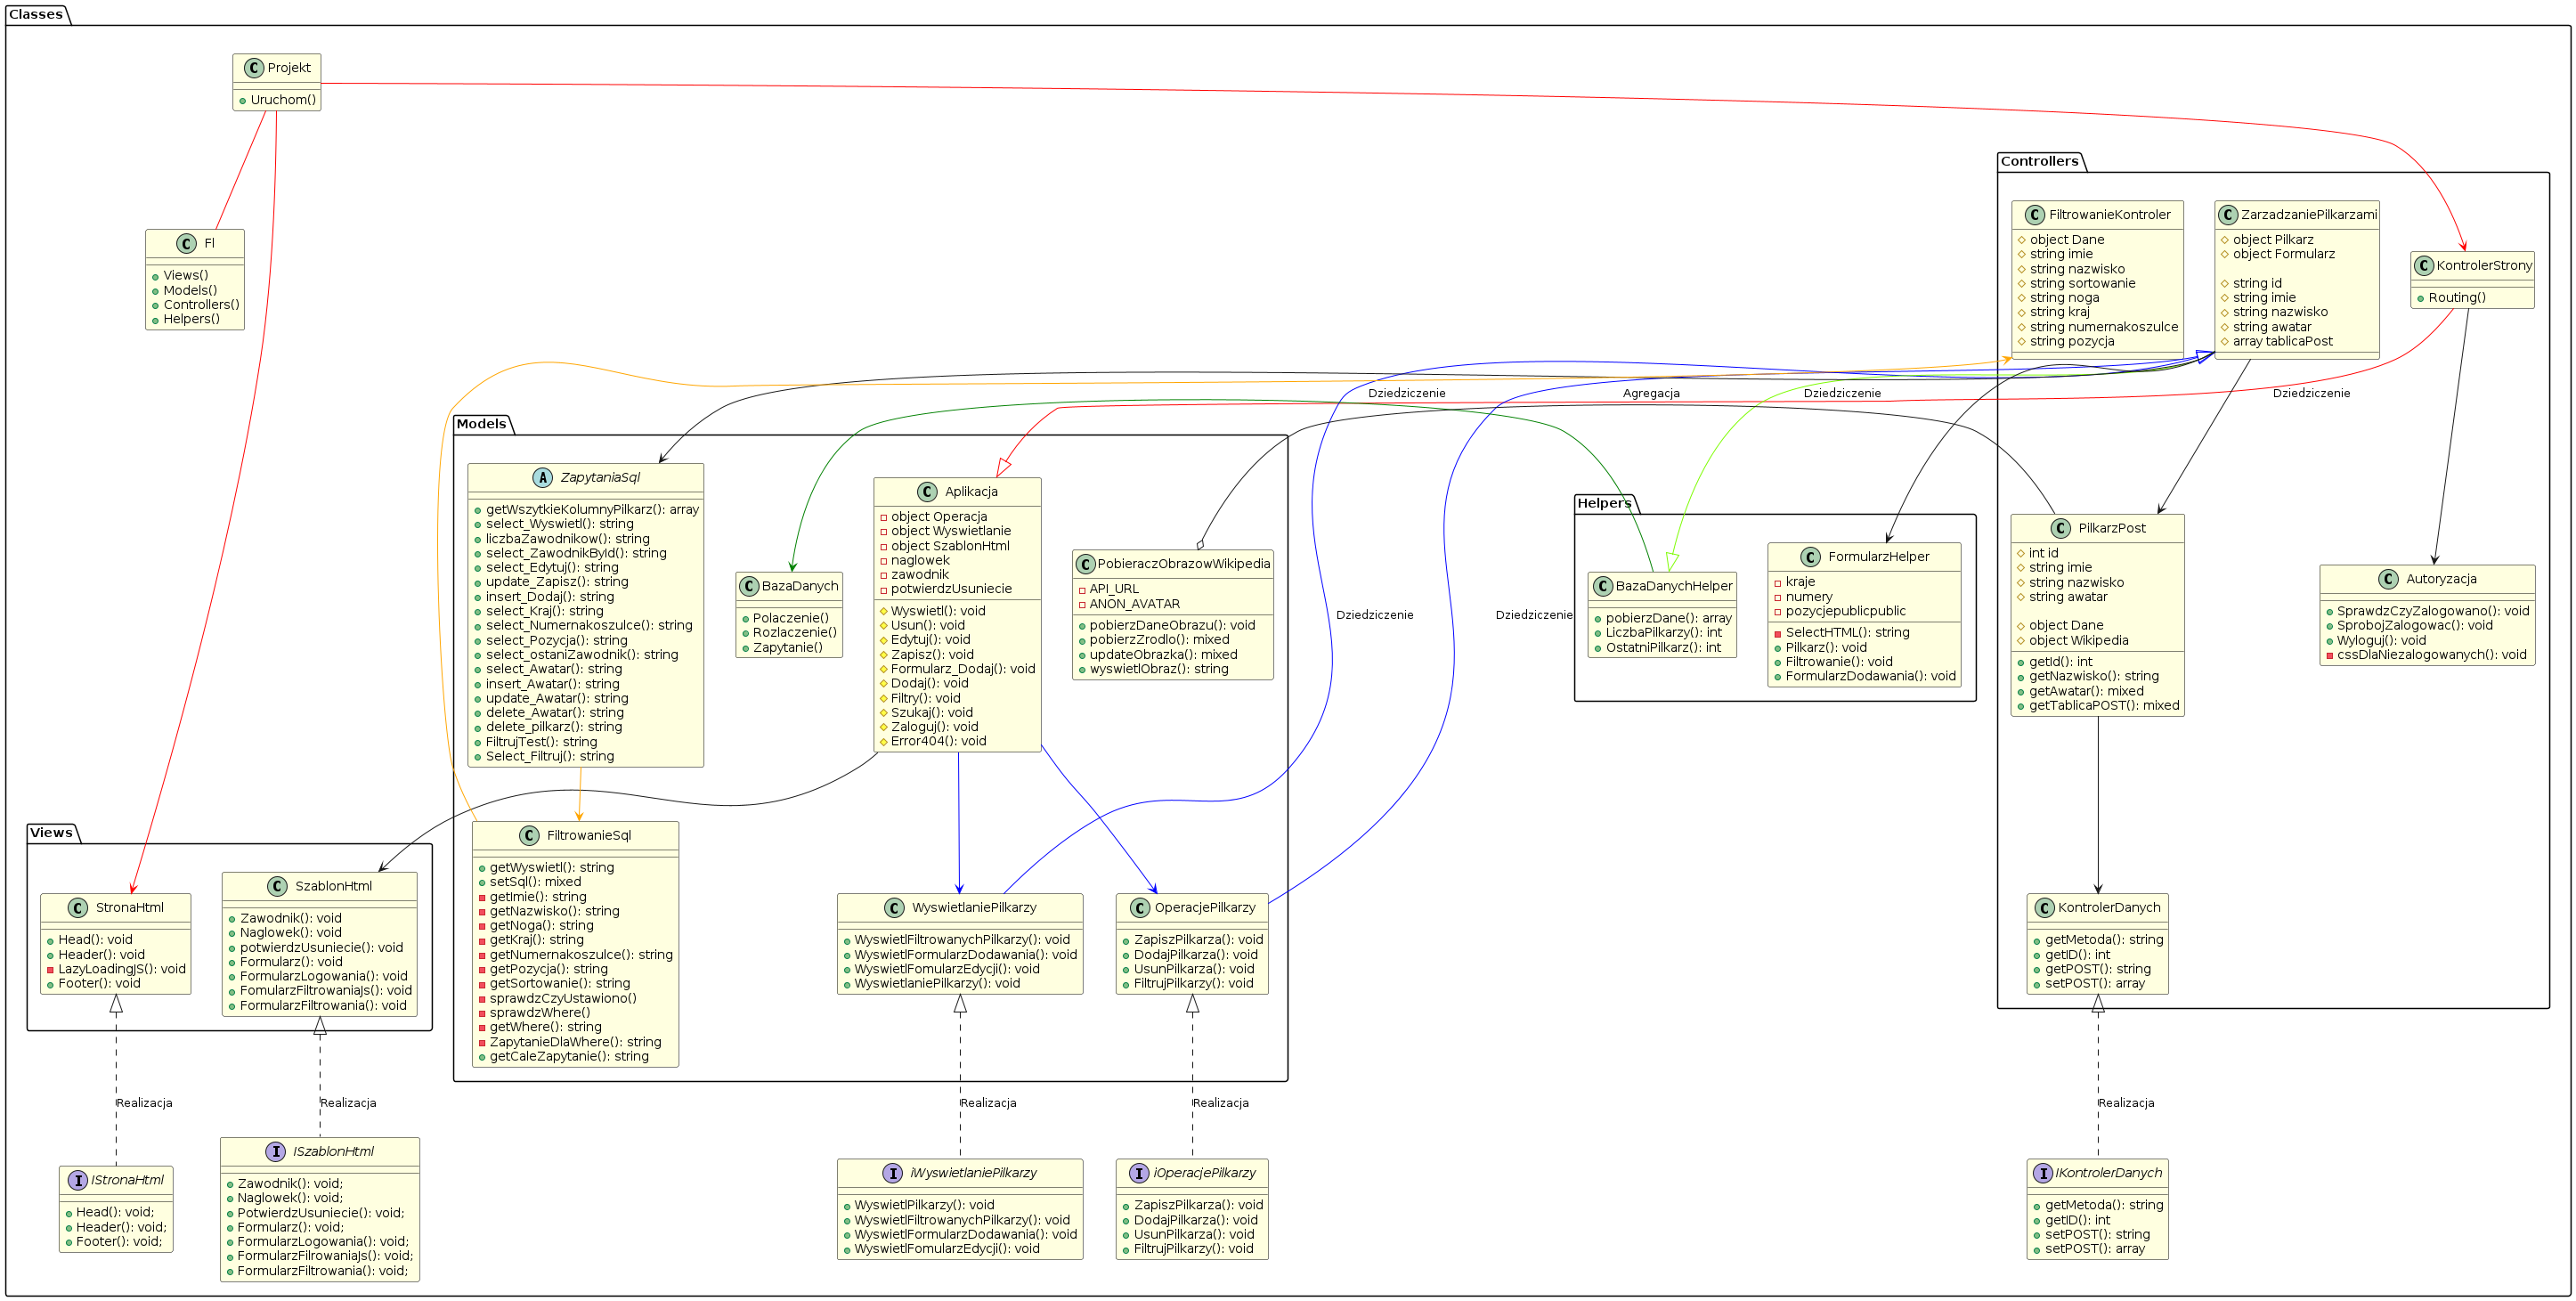
\includegraphics[width=1.0\textwidth]{diagramy/klas.png}
    \caption{Diagram klas - Obraz w pełnej rozdzielczości \url{https://tiny.pl/cnmwh}}                
\end{figure}

\subsection{Opis przeznaczenia klas}
    Klasy są segregowane według modelu \textbf{MVC} i pomocniczych klas opisanych jako \textbf{Helpers}

\subsection{Models}
    \subsubsection{Aplikacja}

    \textbf{Zależności: } 
    Models\textbackslash{}OperacjePilkarzy, 
    Models\textbackslash{}WyswietlaniePilkarzy, 
    Views\textbackslash{}SzablonHtml.\\\\
    
    Stanowi rdzeń całej struktury programu, zarządzając jego ogólnym działaniem, inicjalizacją, oraz kontrolą przepływu danych i interakcji między poszczególnymi komponentami. Jest to kluczowy element, który koordynuje i integruje funkcjonalność innych klas, tworząc spójną aplikację.
    Skupia się na zarządzaniu operacjami związanymi z piłkarzami w kontekście aplikacji. Posiada różne chronione metody , które współpracują z innymi klasami, takimi jak OperacjePilkarzy, WyswietlaniePilkarzy oraz SzablonHtml. Te metody wykonują różne zadania, takie jak wyświetlanie, usuwanie, edytowanie, dodawanie, filtrowanie oraz obsługę błędów w aplikacji związanych z piłkarzami. Klasa ta inicjuje obiekty innych klas w swoim konstruktorze i wykorzystuje je do odpowiedniego przetwarzania i wyświetlania danych w interfejsie użytkownika.\\

    Dostępne metody, pełniają następująca funkcjonalność: 
    \begin{itemize}
        \item \textbf{Wyswietl()} - Wyświetla piłkarzy
        \item \textbf{Usun()} - Usuwa piłkarza
        \item \textbf{Edytuj()} - Wyświetla formularz do edycji
        \item \textbf{Zapisz()} - Zapisuje dane przesłane z formularza
        \item \textbf{Formularz\_Dodaj()} - Wyświetla pusty formularz służący dodawaniu nowego użytkownika
        \item \textbf{Dodaj()} - Dodaje użytkownika do bazy dany na podstawie przesłanych z formularza danych
        \item \textbf{Filtry()} - Wyświetla formularz, który służy do filtrowania
        \item \textbf{Szukaj()} - Wyświetla piłkarzy na podstawie wybranych parametrów
        \item \textbf{Zaloguj()} - Wyświetla formularz logowania
        \item \textbf{Error404()} - Wyświetla status błędu, jeżeli strona nie istnieje
    \end{itemize}
    \lstinputlisting{./src/code_snippets/oop-php/classes/Models/Aplikacja.php}  


    \subsubsection{BazaDanych}
    Odpowiedzialna jest za obsługę połączenia z bazą danych, zarządzanie połączeniem  oraz zapewnienie ogólnej komunikacji z nią. Jest kluczowym połączeniem między aplikacją a danymi przechowywanymi w systemie.\\
    Dostępne metody, pełnią następująca funkcjonalność: 
    \begin{itemize}
        \item \textbf{Polaczenie()} - Ustawienie połączenia z serwerem bazy danych
        \item \textbf{Rozlaczenie()} - Kończy i przerywa połączenie
        \item \textbf{Zapytanie()} - Wykonuje polecenia SQL i pozwala przechwycić rezultat
    \end{itemize}
    Plik konfiguracyjny \textbf{KonfiguracjaDB.php}
    \lstinputlisting{./src/code_snippets/oop-php/KonfiguracjaDB.php} 
    \lstinputlisting{./src/code_snippets/oop-php/classes/Models/BazaDanych.php} 


    \subsubsection{ZapytaniaSql}
    Definiuje i obsługuje generowanie zapytań SQL do bazy danych. Odpowiada za tworzenie struktur zapytań, umożliwiając aplikacji komunikację z bazą w celu pobierania, aktualizacji, usuwania i wstawiania danych.
    Metody zawarte w klasie odpowiadają operacją, jakie wykonuje dane polecenie zawarte w metodzie.
    \lstinputlisting{./src/code_snippets/oop-php/classes/Models/ZapytaniaSql.php} 


    \subsubsection{FiltrowanieSql}
    Jest odpowiedzialna za filtrowanie danych otrzymanych z bazy danych. Zapewnia mechanizmy filtrowania danych, aby  zwracać jedynie pożądane informacje w spójny sposób. Wynikiem końćowym metody \textit{getCaleZapytanie()} jest 
    jedno poprawne zapytanie SQL przekazane do wykonania do bazy danych. 
    \lstinputlisting{./src/code_snippets/oop-php/classes/Models/FiltrowanieSql.php} 

    \subsubsection{OperacjePilkarzy}

        \textbf{Zależności: } 
        Controllers\textbackslash{}ZarzadzaniePilkarzami\\

        Dostarcza zestaw operacji związanych z zarządzaniem danymi dotyczącymi piłkarzy w aplikacji. Obejmuje dodawanie, usuwanie, edycję danych piłkarzy oraz inne operacje z nimi związane.\\
      
        Dostępne metody pełniają następującą funkcjonalność: 
        \begin{itemize}
            \item \textbf{DodajPilkarza()} - Wykonuje zapytanie do bazy danych i dodaje piłkarza
            \item \textbf{ZapiszPilkarza()} - Wykonuje zapytanie do bazy danych i aktualizuje dane na temat piłkarza
            \item \textbf{FiltrujPilkarzy()} - Wykonuje zapytanie do bazy danych, zwraca przefiltrowane wyniki
            \item \textbf{UsunPilkarza()} - Wykonuje zapytanie do bazy danych i usuwa piłkarza
        \end{itemize}
        \lstinputlisting{./src/code_snippets/oop-php/classes/Models/OperacjePilkarzy.php} 


    \subsubsection{WyswietlaniePilkarzy}
        Klasa koncentruje się na prezentacji danych dotyczących piłkarzy. Zapewnia funkcje prezentacji, sortowania, wyświetlania informacji o piłkarzach, dostosowanej do interfejsu użytkownika.\\
        Dostępne metody pełnią następującą funkcjonalność: 
        \begin{itemize}
            \item \textbf{WyswietlaniePilkarzy()} -  Wykonuje zapytanie do bazy danych i wyświetla piłkarzy
            \item \textbf{WyswietlFiltrowanychPilkarzy()} - Wykonuje zapytanie do bazy danych i wyświetla piłkarzy według zastosowanych fitrów
            \item \textbf{WyswietlFormularzDodawania()} - Wyświetla formularz dodawania 
            \item \textbf{WyswietlFomularzEdycji()} - Wykonuje zapytanie do bazy danych i wyświetla formularz do edycji
        \end{itemize}
        \lstinputlisting{./src/code_snippets/oop-php/classes/Models/WyswietlaniePilkarzy.php} 



    \subsubsection{PobieraczObrazowWikipedia}
        Klasa za pomocą otwartego API Wikipedia, pobiera adres URL do głównego zdjęcia piłkarza z artykułu na Wikipedii. Zdjęcie jest pobierane podczas dodawania nowego piłkarza bądź jego edycji i zapisywana w bazie danych w tabeli \textbf{awatar} w postaci linku.\\
        Dostępne metody pełnią następującą funkcjonalność: 
        \begin{itemize}
            \item \textbf{pobierzDaneObrazu()} -  pobiera jako format JSON dane z adresu \url{https://pl.wikipedia.org/w/api.php?action=query&prop=pageimages&format=json&piprop=original&titles=imie_nazwisko}
            \item \textbf{pobierzZrodlo()} - pobiera z tego formatu JSON, link do obrazu
            \item \textbf{updateObrazka()} - w przypadku braku zwraca informacje na temat ścieżki domyślnego obrazu anonimowego użytkownika lub linku do grafiki z serwisu wikipedia
            \item \textbf{wyswietlObraz()} - zwraca tag img, który następnie może zostać wyświetlony.
        \end{itemize}
        \lstinputlisting{./src/code_snippets/oop-php/classes/Models/PobieraczObrazowWikipedia.php} 


\subsection{Controllers}
    \subsubsection{Autoryzacja}
    Obsługuje mechanizm uwierzytelniania użytkowników. Wykorzystuje wbudowany mechanizm sesji w PHP do uwierzytelniania, zapewniając kontrolę dostępu i identyfikację użytkowników w aplikacji.
    \lstinputlisting{./src/code_snippets/oop-php/classes/Controllers/Autoryzacja.php} 


    \subsubsection{FiltrowanieKontroler}
    Odpowiada za filtrowanie danych otrzymywanych od użytkownika. Jest odpowiedzialna za proces sprawdzania, walidacji i filtrowania danych wejściowych (takich jak parametry GET z adresu URL oraz dane POST z formularzy), aby zapewnić bezpieczeństwo i poprawność przetwarzanych informacji.
    \lstinputlisting{./src/code_snippets/oop-php/classes/Controllers/FiltrowanieKontroler.php} 



    \subsubsection{KontrolerDanych}
    Ta klasa ma na celu odbieranie danych od użytkownika z poziomu aplikacji, korzystając z metod GET (parametry z linku) i POST (dane przesyłane z formularzy). Zarządza odbiorem, przetwarzaniem i kontrolą danych, zapewniając ich poprawność i integrację z aplikacją.
    \lstinputlisting{./src/code_snippets/oop-php/classes/Controllers/KontrolerDanych.php} 


    \subsubsection{PilkarzPost}
    Zajmuje się operacjami na danych związanych z piłkarzami, odbierając i przetwarzając informacje przesłane od użytkownika z formularzy POST. Realizuje operacje zapisu danych związanego z piłkarzami do systemu.
    \lstinputlisting{./src/code_snippets/oop-php/classes/Controllers/PilkarzPost.php} 


    \subsubsection{ZarzadzaniePilkarzami}
    Jest klasą, która wykorzystuje klasę pomocniczą BazaDanychHelper do operacji na bazie danych w kontekście informacji o piłkarzach. Ta klasa definiuje podstawowe funkcje i metody obsługi informacji o piłkarzach, wykorzystując metody HTTP - GET i POST do pobierania oraz przesyłania danych.
    \lstinputlisting{./src/code_snippets/oop-php/classes/Controllers/ZarzadzaniePilkarzami.php} 


\subsection{Views}
    Views (pol. Widoki), ta sekcja zawiera metody, które reprezentują warstwę graficzną aplikacji w HTML, CSS i JavaScript. Odpowiada za poprawne wyświetlanie informacji, które zostały uzyskane z bazy danych.
    \subsubsection{StronaHtml}
    Zawiera szkielet strony HTML, taki jak sekcja <head> <body> <footer> czy <header>. Dzięki temu rozwiązaniu można ustawić Podstawowe dane takie jak tytuł strony, autorów, w kilku miejscach na stronie, wczytywana z pliku konfiguracyjnego \textbf{KonfiguracjaApp.php}
    \lstinputlisting{./src/code_snippets/oop-php/classes/Views/StronaHtml.php} 

    \subsubsection{SzablonHtml}
    Klasa zawiera komponenty HTML, które służą do wyświetlania elementów, takich jak card (karta z informacją o piłkarzu), formularze, panel logowania.
    \lstinputlisting{./src/code_snippets/oop-php/classes/Views/SzablonHtml.php} 


\subsection{Helpers}

    \subsubsection{BazaDanychHelper}
    Służy do udostępniania metod wspomagających operacje bazodanowe, takie jak łączenie się z bazą danych, wykonywanie zapytań czy inne operacje związane z bazą danych. 
    \lstinputlisting{./src/code_snippets/oop-php/classes/Helpers/BazaDanychHelper.php} 


    \subsubsection{FormularzHelper}
    Zawiera metody pomocnicze związane z tworzeniem, walidacją czy obsługą formularzy w aplikacji.
    \lstinputlisting{./src/code_snippets/oop-php/classes/Helpers/FormularzHelper.php} 

    
\subsection{Projekt}
    Klasa ta jest ostatecznym elementem programu, posiadającym metodę \textit{Uruchom()}, która integruje Routing, StronęHtml oraz klasę Aplikacja w celu właściwego uruchomienia programu z zachowaniem odpowiedniej kolejności działań. Metoda \textit{Uruchom()} łączy elementy w logiczną sekwencję, umożliwiając kompleksowe działanie aplikacji poprzez współpracę wymienionych składników w spójny sposób.
    \lstinputlisting{./src/code_snippets/oop-php/classes/Projekt.php} 

\subsection{FileLoader}    
    Klasa ma jedynie jedno przeznaczenie: załączenie plików z klasami do projektu. Jej rola polega na importowaniu (łączeniu) różnych plików zawierających klasy, co umożliwia poprawne funkcjonowanie projektu poprzez dostęp do niezbędnych klas i ich metod.
    \lstinputlisting{./src/code_snippets/oop-php/classes/FileLoader.php}  

\subsection{plik - index.php}    
    Ten plik inicjuje metodę \textit{Uruchom()} oraz wykorzystuje klasę FileLoader (skrót Fl) do załączenia plików. Jego głównym zadaniem jest uruchomienie metody \textit{Uruchom()} oraz korzystanie z klasy FileLoader w celu załadowania plików do projektu.
    \lstinputlisting{./src/code_snippets/oop-php/index.php}  